\chapter{Fundamentação Teórica}
\label{cap:fundamentacao-teorica}

\section{Jaguar}
\label{sec:jaguar}

 O Jaguar (figura \ref{Jaguar}) é uma Plataforma Robótica Móvel pertencente a Universidade de Fortaleza – Unifor projetada para aplicações que exigem manobrabilidade robusta e manobrabilidade do terreno. Ele possui quatro braços articulados que convertem o Jaguar aos mais variados tipos de configurações de navegação, facilitando a movimentação e até escalada em vários tipos de terrenos \cite{jaguar}. 

Esse robô também possui video e áudio integrados de alta resolução, bateria, GPS, giroscópio e bússola, tudo para ser controlado remotamente por uma rede sem fio 802.11N \cite{jaguar}. 
Essas características tornam o Jaguar uma excelente plataforma para o uso de inteligência artificial. 


\section{python}
\label{sec:python}

O python é uma linguagem de alto nível orientada a objetos. Ela se tornou tão popular por causa da sua simplicidade, sintaxe clara e concisa e a sua vasta coleção de módulos prontos para o uso \cite{borges2014python}. 

Além de ser utilizada em sistemas operacionais, o python é utilizado em vários softwares para automatização de tarefas (como BrOffice.org, PostgreSQL, Blender, GIMP e Inkscape) \cite{borges2014python}. 

Python é uma linguagem que vem conquistando diversos desenvolvedores e empresas, tal como a Google, a NASA, a IBM, a Embratel e o Serpro. Se comparada a outras linguagens computacionais, provavelmente o python é a que mais oferece bibliotecas para o desenvolvimento de inteligência artificial. Além disso, ela possui uma comunidade de desenvolvedores extremamente ativa, auxiliando o desenvolvimento e aprendizado de novas aplicações nessa linguagem \cite{jonasgranatyr}. 

\section{INTELIGÊNCIA ARTIFICIAL }
\label{sec:INTELIGÊNCIA ARTIFICIAL }

Problemas computacionais sempre foram resolvidos através da programação de
longos códigos, nos quais é especificado cada passo que o computador tem que realizar. Porém, trabalhos que o homem realiza com facilidade pode ser algo bem difícil para ser programado em um computador, como por exemplo o reconhecimento facial, que qualquer acessório ou pequena mudança visual pode dificultar o reconhecimento pelo algoritmo. Essas características, tais como mudança de comportamento, humor e tonalidade da voz são relativamente fáceis de serem percebidas por uma pessoa \cite{lorenafaceli2011inteligencia}. 

%Analise de dados e gráficas são tarefas complexas para serem programadas, principalmente se tiverem que tirar conclusões baseadas nos dados. E, além da complexidade dessas tarefas, é preciso que elas sejam realizadas inúmeras vezes durante um dia. Em alguns casos, o volume de informação é tão grande que se torna impossível de ser analisado por seres humanos \cite{lorenafaceli2011inteligencia}. 
 
Inteligência artificial então é o ramo da computação que procura, por meios computacionais, dar capacidades semelhantes à dos seres humanos para uma máquina, tais como: raciocinar, planejar, resolver problemas, armazenar conhecimento, aprender, perceber e adaptar-se ao meio. \cite{Fernando}.

\section{Aprendizado de Máquina}
\label{sec:aprendizado de máquina}

Estamos em um tempo onde \textit{terabytes} de informações (dados) são criados diariamente. Esses dados podem ser de dois tipos: estruturados (completos sem faltar informação, deixando-o fácil de ser localizado) e não-estruturado (faltando alguma informação nos dados dificultando a sua localização). Se bem trabalhados e analisados, esses dados podem fornecer um grande conhecimento. Cabe então ao algorítimo de Aprendizado de Máquina (ML) trabalhar com esses dados para fazer previsões \cite{pythonmachinelearning}. 

Grandes empresas, como Google, Apple, Amazon, IBM, Microsoft, Facebook e Twitter já usam essa incrível tecnologia. Elas utilizam o \textit{Machine Learning} (Aprendizado de máquina em inglês) para conhecer melhor os seus usuários e fornecer um melhor serviço \cite{pythonmachinelearning}. Um grande exemplo de uso do ML é na analise de sentimentos, onde é possível saber a reação (positiva ou negativa) dos usuários de uma determinada rede social sobre um determinado assunto \cite{sentimentos}.

O algoritmo de \textit{Machine Learning} aprende padrões a partir dos dados entrada juntamente com os seus dados de saída. e pode treinar a máquina para realizar tarefas de forma autônoma. \cite{diferencamachinelearning}.

Em relação ao tipo de aprendizagem, o algoritmo de \textit{Machine Learning} pode ser classificado em três tipos: Aprendizagem Supervisionada (\ref{aprendizadagem supervisionada}), Aprendizagem não supervisionada (\ref{Aprendizagem não supervisionada}) e Aprendizagem por Reforço (\ref{Aprendizagem por Reforço}).

\subsection{Aprendizagem Supervisionada}
\label{aprendizadagem supervisionada}
Nesse tipo de aprendizagem é fornecido para o computador dados rotulados, ou seja, dados de entrada com a sua saída já conhecida. Com isso, é possível prever dados invisíveis ou futuros \cite{pythonmachinelearning}. 
A Aprendizagem Supervisionada pode ser dividida em dois modelos regressão e classificação. No caso da regressão, os dados de entrada são utilizados para criar uma função que gere um valor contínuo. No caso da classificação os dados de entrada são utilizados para mapear os dados de saída em classificações distintas \cite{pythonmachinelearning}. 

\subsection{Aprendizagem não supervisionada}
\label{Aprendizagem não supervisionada}
No caso da Aprendizagem não supervisionada o algoritmo irá trabalhar com dados de entrada nos quais não há praticamente nenhum dado de saída ligado a eles. Ou seja, a máquina terá que gerar uma classificação com os dados de entrada com um determinado padrão entre eles \cite{pythonmachinelearning}. Problemas como esse são normalmente mais complexos principalmente por que não há uma resposta para os dados de teste, tornando assim difícil de avaliar o modelo resultante desse aprendizado.

\subsection{Aprendizagem por Reforço}
\label{Aprendizagem por Reforço}
Através de tentativas e erros, o algoritmo de \textit{Machine Learning} vai procurar uma melhor forma de atuar no ambiente de trabalho para encontrar o sinal de recompensa. Por meio da interação, a máquina procura uma série de ações que levam da melhor maneira possível a recompensa e reduza o erro. Um excelente exemplo dessa aprendizagem é o jogo de xadrez, onde o algoritmo decide, entre uma série de movimentos e o estado do tabuleiro, quais deles vão levar a máquina para vitória e distancia-la da derrota \cite{pythonmachinelearning}.

\section{\textit{Deep Learning}}
\label{deep learning}

Aprendizagem Profunda, em português, é uma forma de aprendizagem de máquina que permite que o computador aprenda através de experiências passadas e compreenda o mundo por uma ideia de hierarquia e conceitos, onde cada nível dessa hierarquia é utilizado para definir outro nível hierárquico. Nesse tipo de aprendizagem não é necessário um operador vistoriando e especificando os conhecimentos necessários para o computador já que ele aprende com experiencias passadas. A hierarquia de conceitos permite que o computador aprenda os conceitos complicados de forma mais simples \cite{goodfellow2016deep}. Então, \textit{Deep learning} (DL) pode ser dito como uma subcategoria do \textit{Machine Learning} que, por meio de algoritmos mais complexos, imita a rede neural do cérebro humano \cite{diferencamachinelearning}.

\textit{Deep Learning} utiliza redes neurais como base do seu algoritmo, porém com muito mais camadas (\textit{Layers}). Foi através dessa subcategoria que tornou-se possível avanços na visão computacional, reconhecimento de fala, processamento de linguagem natural e reconhecimento de áudio.

\section{Redes Neurais Convolucionais}
\label{redes neurais convolucionais}

Rede Neural Convolucional (também conhecida como ConvNet ou CNN) é um tipo de rede neural artificial que pode receber uma imagem de entrada e atribuir importância (com diferentes graus) para vários aspectos ou objetos da imagem e diferenciar um do outro. O pré-processamento de uma rede neural desse tipo é relativamente menor, se comparado aos outros algoritmos de classificação, já que à CNN tem à capacidade de “aprender” o filtro de classificação, enquanto os outros algoritmos necessitam que o filtro seja todo escrito pelo programador\cite{redesneuraisconv,deeplearningbook}.

A primeira proposta de um projeto de rede neural convolucional foi feita em 1988, por Yann LeCun. Seu nome era \textit{LeNet} e era utilizada para o reconhecimento de características numéricas. Ela foi de grande utilidade para impulsionar o campo de pesquisa de \textit{Deep Learning} \cite{redesneuraisconv}.

Os algoritmos de CNN podem dar capacidade ao computador de ver o mundo como um ser humano, conseguindo distinguir diferentes objetos e aspectos da imagem em análise. À figura  \ref{keras_exemple} mostra um excelente exemplo disso, no qual  o algoritmo consegue, com alta taxa de precisão, distinguir os diferentes conteúdos da imagem \cite{conv1,conv2}.

\begin{figure}[H]
	\centering
	\Caption{\label{keras_exemple} Exemplo de reconhecimento de Objetos de uma CNN}
	\UNIFORfig{}{
		\fbox{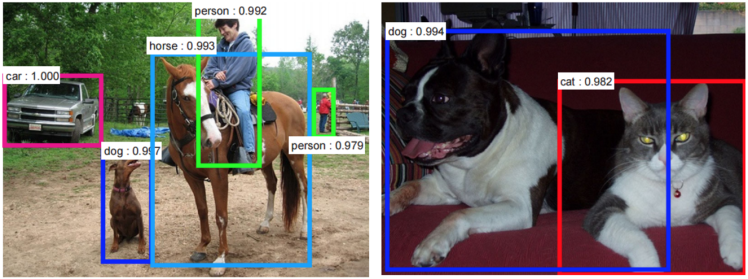
\includegraphics[width=15cm]{fig/keras_exemple.png}}
	}{
		\Fonte{\cite{conv2}}
	}	
\end{figure}

Existem diversas bibliotecas que realizam à implementação de uma Rede Neural Convolucional: \textit{Caffe, MatConvNet, Theano, Torch}. Para esse projeto foi utilizado o \textit{Keras} para o desenvolvimento da Rede Neural, que é uma API de alto nível desenvolvido em python e baseado no \textit{Tensorflow}, biblioteca de aprendizado de máquina  e de código aberto desenvolvida pelo \textit{Google Brain}, em 2015 \cite{redesneuraisconv,keras,tensorflow}.

A arquitetura de uma \textit{ConvNet} é semelhante ao padrão de conectividade dos neurônios dos seres humanos, sendo inspirada na organização do Cortex. \cite{conv1}

 As CNNs possuem diversas comandas, mas há sempre três principais: convolucionais, \textit{pooling} e totalmente conectada. A camada convolucional possui diversos neurônios que tratam de aplicar um filtro em uma determinada parte da imagem. A camada de \textit{pooling} trate de reduzir o tamanho da imagem e fazer a ativação dos pixels mais significativos e a camada totalmente conectada faz a classificação. A figura \ref{exemplo_cnn} mostra uma ilustração de uma CNN.

\begin{figure}[H]
	\centering
	\Caption{\label{exemplo_cnn} Ilustração de uma CNN}
	\UNIFORfig{}{
		\fbox{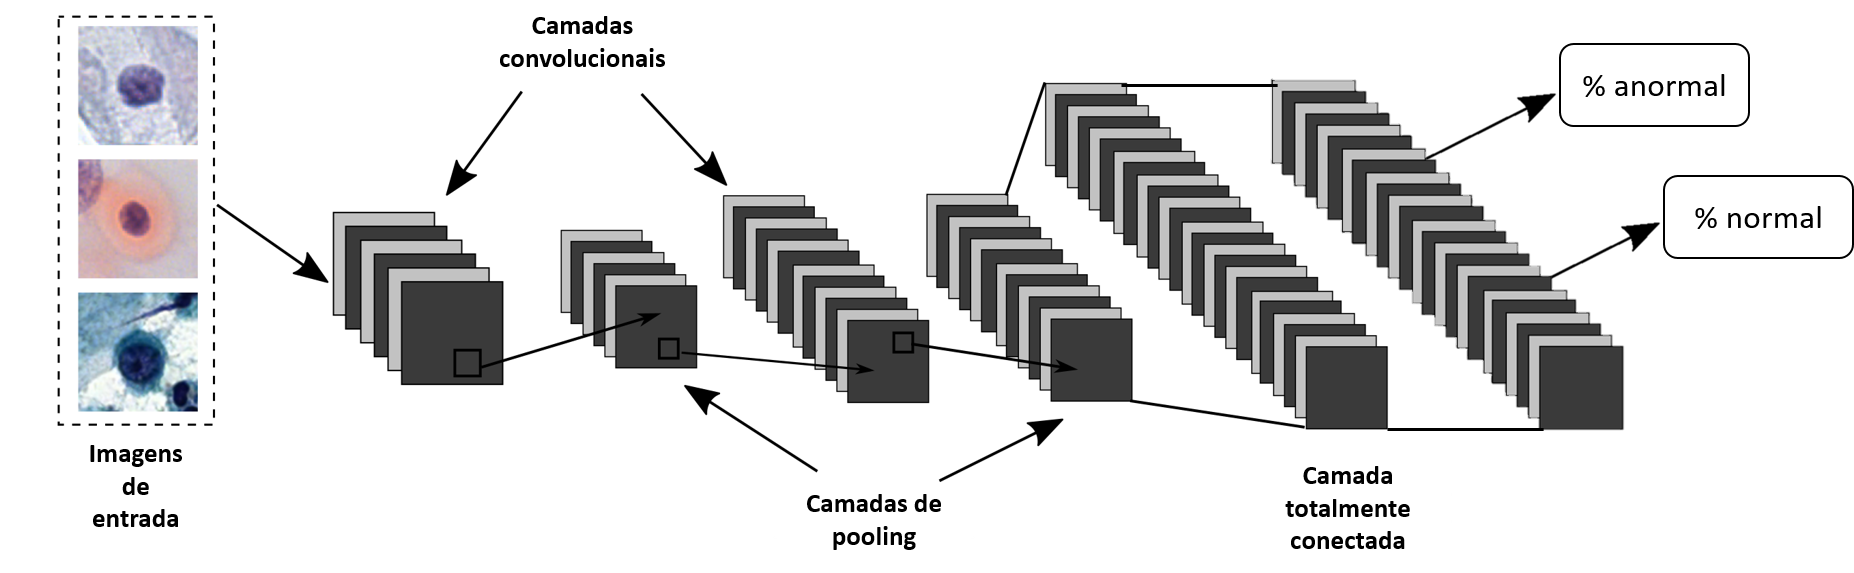
\includegraphics[width=15cm]{fig/exemplo_CNN.png}}
	}{
		\Fonte{\cite{redesneuraisconv}}
	}	
\end{figure}

O volume de entrada que o algoritmo de CNN irá trabalhar é uma imagem. Para entender o funcionamento do algoritmo é preciso primeiramente entender o que é uma imagem na visão computacional\cite{conv2}. 

Basicamente é possível dizer que uma imagem é uma matriz de valores de pixel. Cada valor dessa matriz possui três canais: vermelho, verde e azul, no qual cada um possui um número de 0 a 255 para assim poder formar as cores de cada pixel da imagem. Para imagens em preto e branco existem apenas um canal que também vai de 0 á 255, porém apenas na escala de cinza. 
Com essa visão básica de como é formado uma imagem, é possível compreender como cada uma das camadas da rede neural trabalham em cima dela \textit{resolucao}.

\subsection{Camada Convolucional}

É a primeira camada da CNN. Sua função reduz o tamanho da imagem sem perder suas principais características que são fundamentais para a predição. Para isso, é possível utilizar quantas camadas for necessário \cite{freecodecamp}. É uma camada que consiste em um conjunto de filtros (também conhecidos como \textit{kernels}), que são configurados pela própia CNN enquanto ela vai recebendo dados de entrada, nos quais eles recebem como entrada um arranjo tridimensional, também chamado de volume. Nessa camada nem sempre os neurônios são conectados a todos os neurônios da camada seguinte, como na Rede Neural. Eles se conectam à apenas uma pequena região do mesmo. Conforme a imagem passa por cada camada convolucional ela vai reduzindo assim como o seu filtro \cite{freecodecamp, conv2}.
 
 Uma imagem retirada de um video \textit{Full HD} tem uma resolução de 1920 x 1080 \textit{pixels}, ou seja, 1920 \textit{pixels} na largura e 1080 \textit{pixels} na altura, no qual cada um desses \textit{pixels} há três canais de cores com 256 tonalidades para cada um \cite{resolucao}. Por questões de didáticas, será utilizado um exemplo mais simples de resolução 5 x 5 e apenas um canal de cor com 2 tonalidades.
 \begin{figure}[H]
	\centering
	\Caption{\label{filtro1} Volume de entrada e o Filtro}
	\UNIFORfig{}{
		\fbox{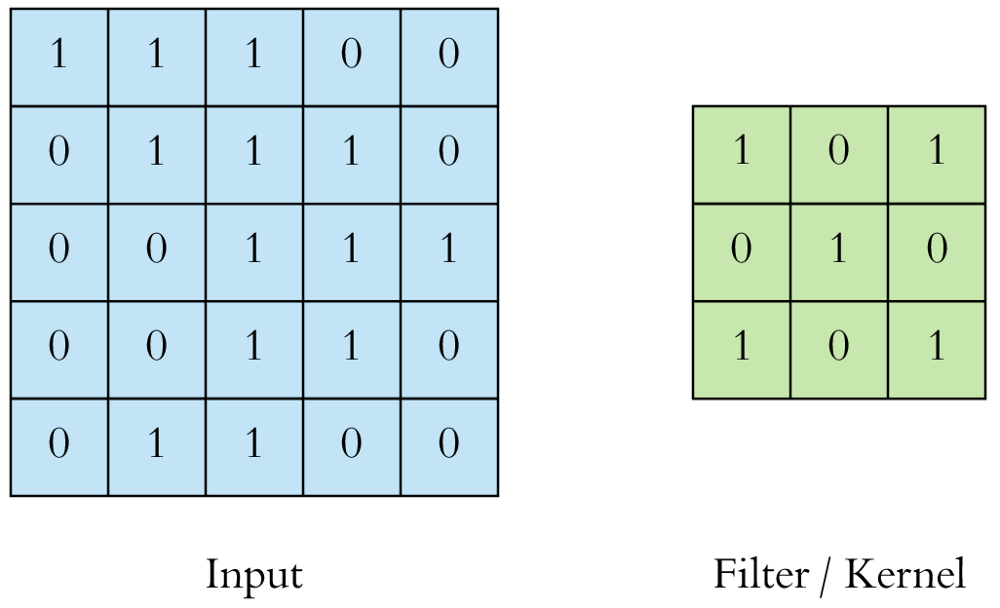
\includegraphics[width=12cm]{fig/filtro3.png}}
	}{
		\Fonte{\ref{freecodecamp}}
	}	
\end{figure}

Na figura \ref{filtro1} temos a Imagem de entrada representada pelo \textit{Input}, onde cada \textit{pixel} é representado por um quadrado da figura e o seu filtro representado por \textit{Filter/Kernel}. O filtro irá passar sobre essa imagem, da esquerda para direta, fazendo o cálculo da matriz da imagem com a matriz do filtro, resultando num mapa de recursos (ou \textit{feature map}), como mostrado na figura \ref{filtro2} \cite{conv2}.

 \begin{figure}[H]
	\centering
	\Caption{\label{filtro2} Mapa de recursos 1}
	\UNIFORfig{}{
		\fbox{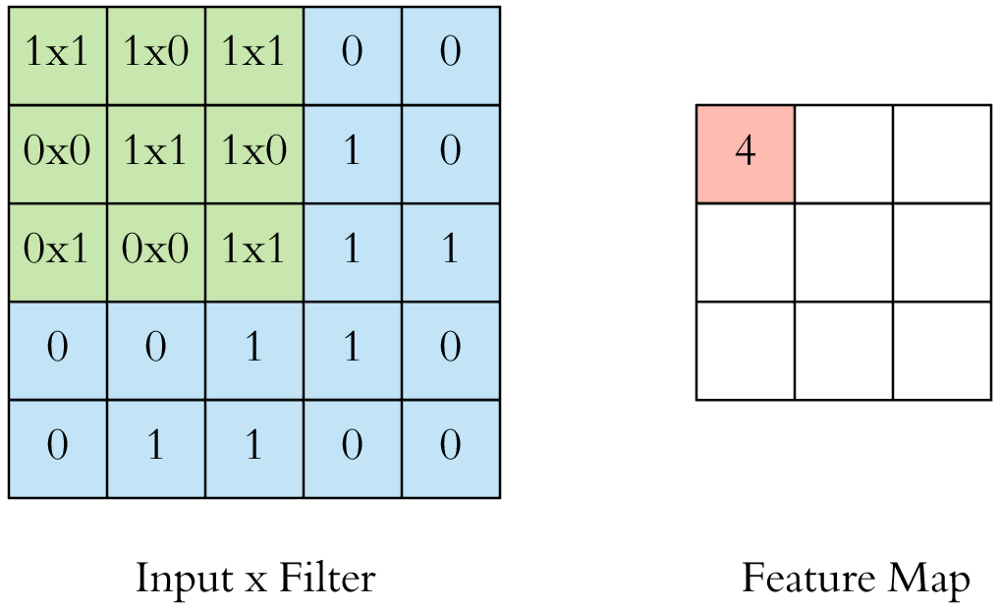
\includegraphics[width=12cm]{fig/filtro2.png}}
	}{
		\Fonte{\cite{freecodecamp}}
	}	
\end{figure}

O filtro percorre, da esquerda para direta e de pixel por pixel, fazendo a multiplicação dos \textit{pixels} da imagem pelos \textit{pixels} do filtro e somando o resultado para criar o mapa de recursos que tem uma linha de pixel a menos em cada um dos seus lados. Esse movimento é repetido linha por linha da imagem de entrada. O resultado Final é mostrado na figura \ref{filtro3} \cite{conv2, freecodecamp}.

 \begin{figure}[H]
	\centering
	\Caption{\label{filtro3} Mapa de recursos 2}
	\UNIFORfig{}{
		\fbox{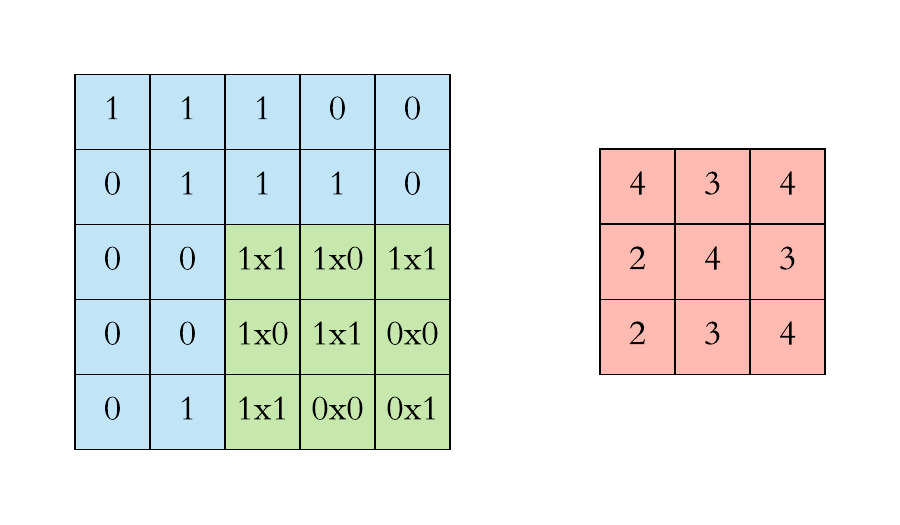
\includegraphics[width=12cm]{fig/filtro4.jpg}}
	}{
		\Fonte{\cite{freecodecamp}}
	}	
\end{figure}

Os filtros podem possuir diferentes valores, gerando assim diferentes efeitos convolucionais. Com isso é possível realizar operações como detecção de borda, nitidez e borrão com apenas uma mudança de valores numéricos da sua matriz. A figura \ref{filtro4} mostra exemplos de algumas operações. Elas são descritas na primeira coluna (identidade, detecção de bordas, aguçamento e borrão, em ordem). Na coluna do meio tem a matriz do filtro e o resultado convolucional na ultima coluna. Os  valores dos filtros são aprendidos pela CNN, mesmo ainda sendo preciso especificar alguns parâmetros pelo programador como número, tamanho, arquitetura do filtro \cite{conv2, aprendizadoDeMaquinaDivertido}.

\begin{figure}[H]
	\centering
	\Caption{\label{filtro4} Diferentes tipos de Filtros}
	\UNIFORfig{}{
		\fbox{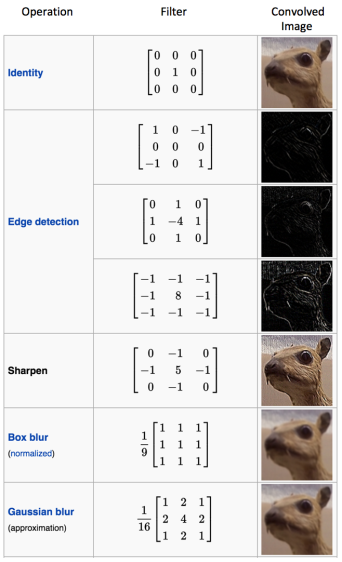
\includegraphics[width=10cm]{fig/tiposdefiltros.png}}
	}{
		\Fonte{\cite{conv2}}
	}	
\end{figure}

O resultado final da convolução, o \textit{feature map} é controlado por três parâmetros:
\begin{description}
    \item[Profundidade:] é o número de filtros usado para a convolução.
    \item[\textit{Stride:}] é o número de \textit{pixel} que o filtro vai percorrer por vez. Por exemplo: se o \textit{Stride} for igual a 1, o filtro vai percorrer apenas 1 pixel por vez.
    \item[\textit{Zero-padding:}] em alguns casos é preciso preencher a borda da matriz de de entrada (a imagem) com zeros para poder controlar o tamanho do mapa de características. 
\end{description}

Ao final de cada operação de convolução também é comum utilizar uma função de não-linearidade, a ReLU. Sua função é substituir todos os \textit{pixels} negativos por zero do mapa de recursos. Então, a Unidade Linear retificadora (ReLU) introduz a não linearidade no resultado final já que a maioria dos dados de entrada reais são não lineares \cite{conv2}.
A Figura \ref{filtro6} mostra um excelente exemplo da aplicação dessa função, onde a imagem da direita é o resultado depois da aplicação do filtro.

\begin{figure}[H]
	\centering
	\Caption{\label{filtro6} Aplicação do Filtro ReLU}
	\UNIFORfig{}{
		\fbox{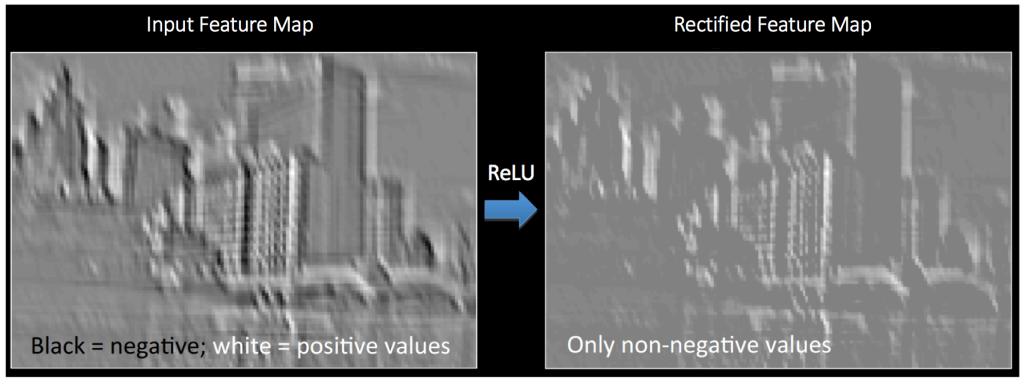
\includegraphics[width=16cm]{fig/relu.png}}
	}{
		\Fonte{\cite{conv2}}
	}	
\end{figure}

Para esse projeto foi utilizado a função de ativação ELU (Unidade Linear Exponencial, ou ingles, \textit{Exponential Linear Unit}). Ela converge mais rapidamente para o zero e possui resultados mais precisos.

Em relação ao ReLU, ela possui uma constante extra positiva, chamada de alfa. Ela também difere do ReLu pela sua suavisão que é mais lente e bem menos acentuada. Podemos ver isso no gráfico da figura \ref{elurelu} \cite{elu}.

\begin{figure}[H]
	\centering
	\Caption{\label{elurelu} Função Elu x ReLU}
	\UNIFORfig{}{
		\fbox{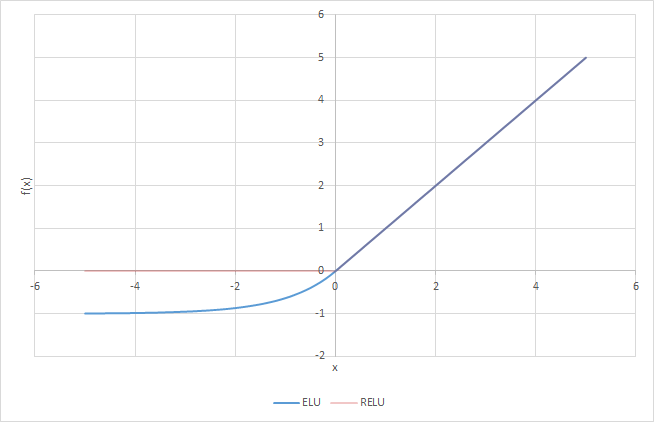
\includegraphics[width=15cm]{fig/elurelu.png}}
	}{
		\Fonte{\cite{elu}}
	}	
\end{figure}

\subsection{Camada de \textit{Pooling}}

A função da camada de \textit{pooling} (também chamada de subamostragem ou \textit{downsampling}) é reduzir a dimensão do mapa de recursos mantendo as informações mais importantes. Podemos ter a soma, a média ou \textit{Max Pooling}, que é a mais popular e também utilizada nesse trabalho. Essa ultima funciona definindo uma janela de \textit{pixels} (por exemplo, uma janela 2x2 onde ela "visualiza" apenas 4 \textit{pixels} do mapa de amostragem) e seleciona o maior deles para montar outro mapa de recursos, como é mostrado na figura \ref{maxpool}. Essa função se aplica por toda a imagem \cite{freecodecamp}.

\begin{figure}[H]
	\centering
	\Caption{\label{maxpool} Aplicação do \textit{Pooling}}
	\UNIFORfig{}{
		\fbox{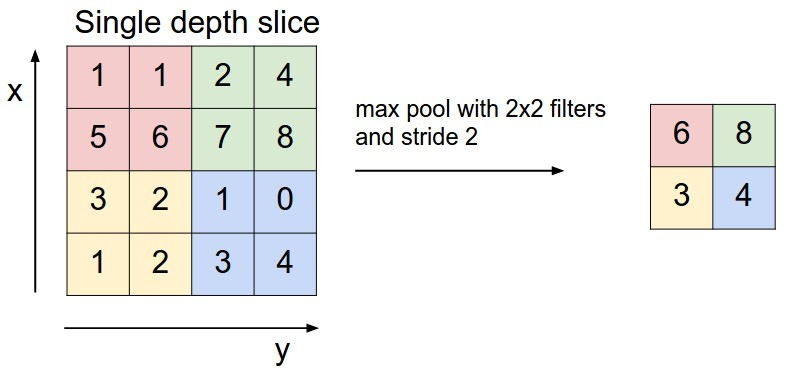
\includegraphics[width=15cm]{fig/maxpool.jpg}}
	}{
		\Fonte{\cite{CS231n}}
	}	
\end{figure}

O resultado da aplicação desse camada é mostrado na figura \ref{pool} (lembrando que já foi aplicado a convolução e ativador ReLU na imagem).

\begin{figure}[H]
	\centering
	\Caption{\label{pool} Exemplo de \textit{Pooling}}
	\UNIFORfig{}{
		\fbox{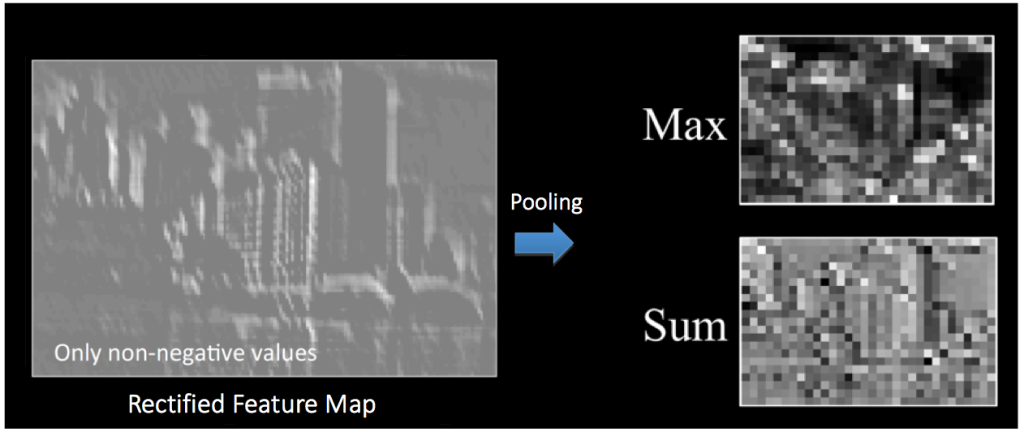
\includegraphics[width=15cm]{fig/pool.png}}
	}{
		\Fonte{\cite{conv2}}
	}	
\end{figure}

\subsection{Camada \textit{Fully Connected}}

Camada totalmente conectada, em português, é uma camada onde todos os neurônios da camada anterior estão totalmente conectados a todos os neurônios da camada posterior. Seu objetivo é classificar as imagens de entrada nos vários grupos determinados pelo \textit{dataset}. Essa é etapa final da predição, onde ela irá retornar um valor para o usuário entre 0 (0\% de probabilidade) e 1 (100\% de probabilidade) referente a cada um dos \textit{datasets}. A figura \ref{exemploCNN} mostra, na sua extremidade direita, o percentual de probabilidade de ser cada um dos \textit{datasets} inseridos. Pode-se observar que o \textit{boat} (barco) tem a maior probabilidade, sendo 0,94.\cite{conv2, aprendizadoDeMaquinaDivertido}. 
Lembrando que esses são as camadas básicos de uma CNN, mas não necessariamente elas precisam sempre seguir essa Ordem. Na figura \ref{exemploCNN}, por exemplo, há duas camadas Convolucionais com ReLU e \textit{Pooling} para no final haver duas camadas totalmente conectadas \cite{conv2}.

\begin{figure}[H]
	\centering
	\Caption{\label{exemploCNN} Exemplo de Rede Neural Convolucional}
	\UNIFORfig{}{
		\fbox{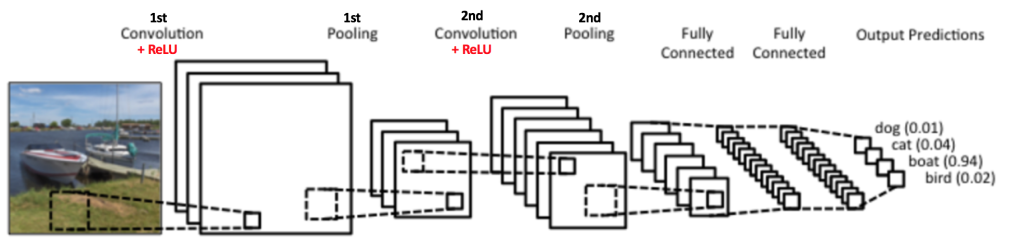
\includegraphics[width=16cm]{fig/exemploCNN.png}}
	}{
		\Fonte{\cite{conv2}}
	}	
\end{figure}